%!TEX root = ../dissertation.tex

\chapter{Solution}
\label{chapter:solution}


\section{Overview}
Our solution is comprised of two main components, a web page, responsible for the \gls{ui} of the programming environment, and a remote CAD service, responsible for offering an \gls{api} for running programs in \glspl{cad} installed in user's computers to the rest of the system.

Please note that it is only ever needed to install the server when the architect is finally ready to get the program's results on a \gls{cad}.
Like so, the server can just be installed in the computer that actually has the \gls{cad} installed while the rest only accesses the web page.
Once installed and started, the web page can start requesting operations to be executed in the available \glspl{cad}.

programming environment, cad export, program persistence(not implemented)

Figure~\ref{fig:arch:overview} shows the relationships between these components. {\it arrows indicating interactions between them?}

\begin{figure}
  \centering
  
\includegraphics[width=12cm]{./images/architecture_overview}
  \caption{An overview of the solution's architecture.}
  \label{fig:arch:overview}
\end{figure}

In the rest of this chapter, we describe the details of each of these components, how they interact with each other and the problems faced when implementing them.


\section{Web page}
The web page is main contact point between the architect and our solution.
Using it, he will be able to work on \gls{gd} programs, share them with colleagues and ultimately deliver results.

It acts as the \gls{ide} and like so implements the features that were discussed earlier.
For that purpose, it comprises a text editor for editing programs and a 3D view for displaying results of that program, as seen in Figure~\ref{fig:page:view}.

\begin{figure}
  \centering
  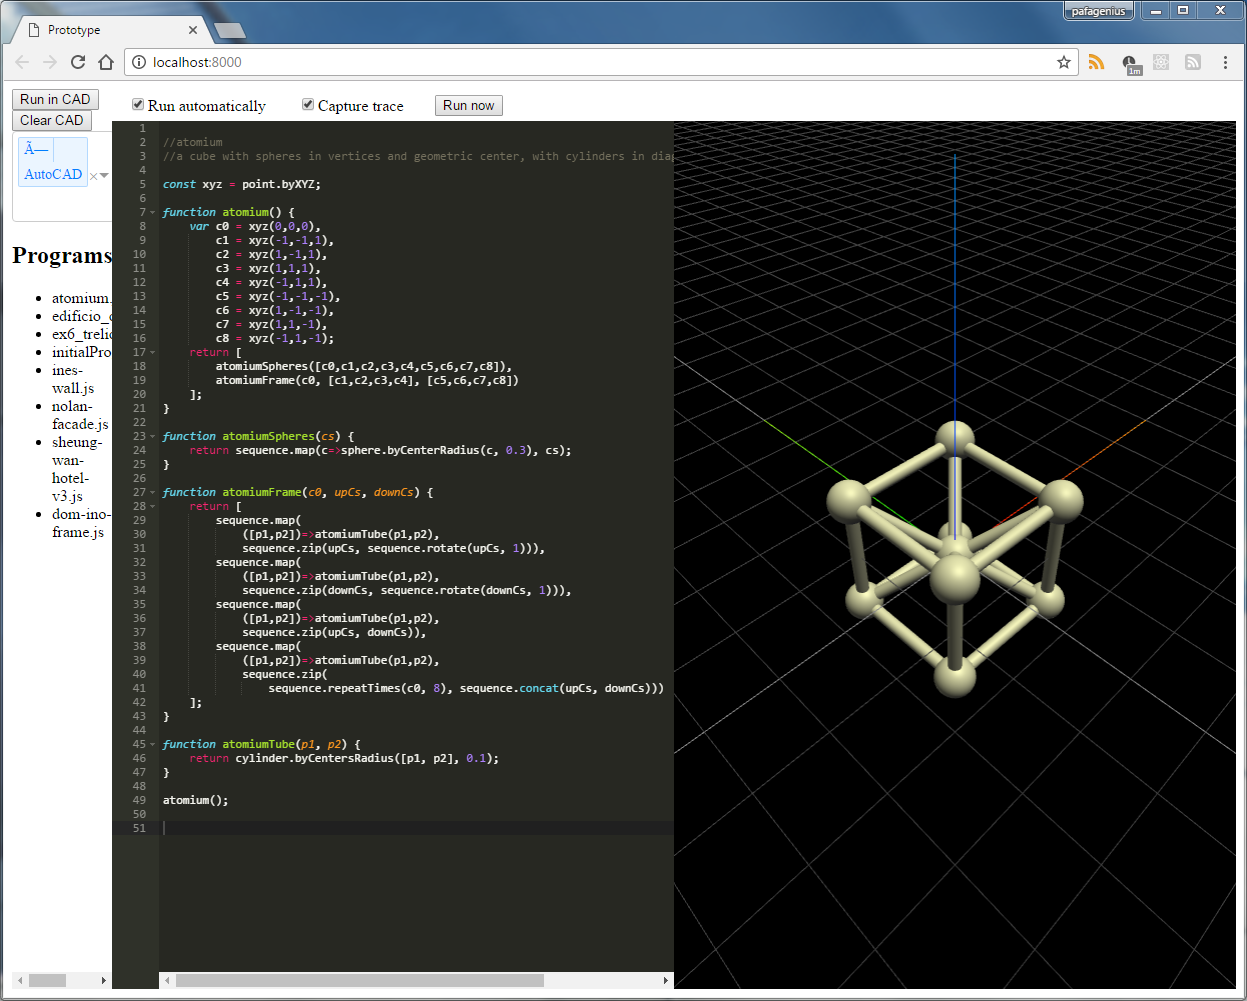
\includegraphics[width=12cm]{./images/webpage_view}
  \caption{An example view of the web page.}
  \label{fig:page:view}
\end{figure}

A text editor and a 3D view by themselves do nothing more than display text and 3D objects.
To make the \gls{ide} actually helpful several other parts had to be implemented.

\subsection{Adjusting Literals}
When a value, such as a number, is typed directly into a program's source code, it is called a literal value, or simply by literal.
When experimenting with a \gls{gd} program, architects find themselves repeatedly adjusting literals that were hardcoded into the program.
This is usually done by retyping parts of the literal's text to higher or lower digits.

Editing literals this way often leads to errors since it is easy to mistype some characters.
One can increase their value by an order of magnitude if, by mistake, he inserts one character without removing another.
When increasing them in steps, different hand movements are required when there is carry over, yet again increasing both the likelihood of mistyping and the time it takes to make the changes.
These errors get amplified when the programming environment provides real time feedback and, like so, begins re-executing the program before the error is corrected leading to reduced \gls{ui} responsiveness.

There are several ways we can extend the user interface to make this more user friendly.
None of them rely on manually replacing digits.
They have a simpler mapping to the user's intent.
The following list describes some of them:

\begin{description}
  \item[Virtual joystick] Clicking on a literal will display a virtual joystick close to it. When clicked and dragged, it changes the value repeatedly over time, being faster or slower depending on how much the handle is moved from its center.
  \item[Click and drag] Clicking and dragging on a literal will change it according to how much the pointer moved from the starting position.
  \item[Sliders] Clicking on a literal will display a slider. Dragging the slider's handle will change the literal depending on how much the handle is moved from the center of the slider. The slider can have different scales, linear or non-linear, to map the center-handle distance to the amount of change for the literal.
  \item[Keyboard shortcuts] Pressing key combinations while having a literal selected, or the text editor's caret on it, will increment or decrement it.
\end{description}

We chose to implement the ``Click and drag'' method in our solution.

\subsubsection{Implementation}
To implement this behavior, we need to focus on the program editor.
This is where the relevant information is.

The behavior starts when the user presses a mouse button while the pointer is over a numerical literal.
If it is indeed a numerical literal, we setup an event listener that will update the literal every time the pointer moves until the mouse button is released.

To check that the pointer is over a numerical node, we use the pointer position and the \gls{ast} of the current program with location data.
Since the program will change during the behavior, we keep the path taken through the \gls{ast} to the numerical literal.
We also keep the starting pointer position as a reference for calculating the new literal value when the mouse is moved.

We update the literal by changing the portion of the source text that it refers to to the text representing the new value.
The new value has the same number of fractional digits as the original literal.
To get the new value, we first extract the number of fractional digits and an integer containing the literal's digits and sign (ignoring the decimal point) from the literal's source text.
Afterwards, we add the horizontal distance between the starting point and the current pointer position to the number.
Finally, we convert it back to text and re-add the decimal point.

\subsubsection{Use case}
To hint that a literal is adjustable, the pointer changes to ``$\Leftrightarrow$''.

\subsection{Getting results / What is a program?}
Before a program can be run, the programming language has to be defined.
In our solution, we decided that it would be best to use JavaScript as it was thought for designers and also because of its current performance.

However, there is a question: how do we get results from a program so we can display them?
Our solution uses the values of the top-level expression statements of the program as its results.

There are other alternatives that could have been used.
For example:
\begin{description}
  \item[Special entry point] Like in OpenJSCAD, we could require that every program must define a function with a special name (e.g. ``main''). Upon being called, that function produces the result of the program.
  \item[Display function] Another way to get results from a program is giving access to an output function to the program. During its execution, the program then calls this function, maybe several times, to produce its output.
  \item[Imperative primitives] A third way to get results is by adding a side-effect to the 3D object producing functions/primitives. Apart from creating the object, they also add it to the program's results. This is a special case of the previous item where all primitives are display functions.
\end{description}

\subsection{Handling traceability}
As was said previously, letting the architect see the connection between the program and its results lets him go a long way towards understanding the program.
If the programming environment takes care of tracking the relation between the program and the results, the architect only needs to ask for the relation instead of having to track it by himself, freeing his mind to think about the problem.

There needs to be a way to give the architect quick access to the relation being tracked by the environment.
To do this, our solution highlights certain parts of the program and  its results when the pointer is on either one.
More specifically, when the pointer is over a part of the program, it highlights all the results that it produced;
when the pointer is over a part of the results, it highlights the part of the program where it was created.
Figure~\ref{fig:trace:example} shows an example for both of this cases.

\begin{figure}
  \centering
  
\includegraphics[width=12cm]{./images/traceability_example}
  \caption{Two examples of the traceability mechanism. The first from program to results and the second from results to program.}
  \label{fig:trace:example}
\end{figure}

Currently our solution only tracks the results produced by calls to functions.
This was a compromise (though, not tested) since keeping track of traceability is an additional task that needs to be performed while running the program.

There are other ways for showing the relation between the program and its results.
We will describe some of them next.
\begin{description}
  \item[Timetable] As described in {\it Learnable Programming}\cite{victor2012learnable}, making things visible makes them more real to the programmer. Timetables proposed as a way to visualize the control flow of programs. They act as a map of the program's execution. By seeing the control flow, it is easier to see what the program does and it is easier to point at interesting locations. Timetables provide better navigation inside a program's execution.
  \item[Display data] Also described in {\it Learnable Programming}\cite{victor2012learnable}, displaying data would increase the amount of traceability the system provides. Apart from being able to see the control flow and the 3D results, seeing the other values (e.g. numbers, booleans) used throughout the program would give the programmer a more complete view of the execution.
\end{description}

\subsection{Providing primitive/predefined bindings}
\label{sub:provide:predefs}
Any program needs to anchor itself in some functionality already provided by its host environment.
It is this functionality that enables the program to do interesting work.

But how does our solution do this for programs written by architects?
We do this by defining all predefined functionality in a JavaScript module and then providing it to the function that represents the program as a parameter.
Afterwards, we also add some code to the beginning of the program that will declare each primitive and extract the corresponding functionality from that parameter.

\subsection{Running programs}
One of the fundamental parts of the programming environment is that it runs programs.

After having a program at hand, we have to instrument it so that we can collect its results in addition to traceability data, like the return values of function calls.

To run a program, the \gls{ide} starts by getting the \gls{ast} of the program so it can analyze it to produce an instrumented version that will record all the information it needs.

We have to keep a mapping between the nodes that comprise the \gls{ast} and the information that is going to be recorded.

The instrumentation does two things:
\begin{itemize}
  \item All call expressions are replaced with an \gls{iife} that performs the call, records its result and returns it to keep the semantics of the program.
  \item All expressions in the program's top-level are replaced with a call to a function that records their result.
\end{itemize}

After this step a new function is created whose body is the instrumented program.
The predefined functions are provided as parameters to this new function.

Finally, the newly created function is called and, afterwards, the recorded information is made available to the rest of the \gls{ide}.


\section{Remote CAD Service}
As previously said, there is also a ``remote CAD service'' as part of the solution.
This service is responsible for enabling programs to take effect on the \glspl{cad} that architects have installed on their computers.
This way, they can share their work with team member that use software that expect files from traditional \glspl{cad}.

To make this possible, the service requires that the architect run a software in the computer he wants his program to take effect.
This software connects to the ``remote CAD service'' and waits for requests to make shapes in the \glspl{cad} installed in the computer.

\subsection{Implementation}
We implemented the software as a small Racket server.
It expects to receive HTTP requests for adding shapes to the currently selected \glspl{cad}.
It also receive requests for specifying what \glspl{cad} should the shapes be added.

Instead of implementing the connection and communication with the \glspl{cad} installed in the computer ourselves, we used Rosetta as an intermediate.
This way, we only had to concern ourselves with correcting the semantic differences between Rosetta's \gls{api} and the ``remote CAD service'''s \gls{api}.

Because of the cross domain restrictions imposed by web browsers for \gls{ajax} requests, we chose to temporarily host the web page that contains the \gls{ide} in this server.
It is a quick and dirty way to test the communication between the page and the ``remote CAD service''.

%Design principles / Guiding ideas
%- Ideas based on observations from related work?

%Architecture - Show the overview of the architecture
%- Web page + remote CAD service

%Web page
%- Architecture
%- Page Layout
%- Features / What needs to be done by the IDE?
%   - Discussion + Decision
%   - Implementation
%- Problems
%   - Adjusting source code values
%   - Instrumenting and running programs
%     - Getting results / What is a program?
%     - Providing primitives/predefined bindings
%     - Handling traceability
%   - (Running programs blocks the UI)
%   - Displaying 3D results

%Remote CAD service
%- Architecture
%- Problems
%   - Supporting multiple CADs
%   - Defining the API

%Problem: Handling CAD communication
